\begin{figure}[ht!]
\centering
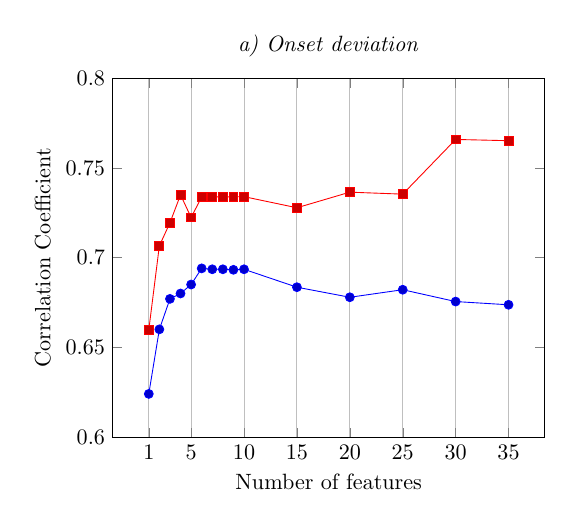
\begin{tikzpicture}[scale=0.8]

\begin{axis}[legend style={font=\scriptsize},
		title={\textit{a) Onset deviation}},
        ylabel={Correlation Coefficient},
        xlabel={Number of features},
        ymin=0.60,ymax=0.80,
        xtick={1,5,10,15,20,25,30,35},
        xmajorgrids]

    \addplot coordinates {(1,0.624) (2,0.660) (3,0.677) (4,0.680) (5,0.685) (6,0.694) (7, 0.6935)  (8, 0.6935) (9,0.6932) (10,0.6935) (15,0.6835) (20, 0.6779)  (25, 0.6821) (30, 0.6755) (35, 0.6737)};
    
    \addplot coordinates {(1, 0.6597) (2, 0.7066)  (3, 0.7194) (4, 0.735) (5, 0.7224) (6, 0.7338) (7, 0.7339) (8, 0.7339) (9, 0.7339) (10, 0.734) (15, 0.7278) (20, 0.7365) (25, 0.7354) (30, 0.7659) (35, 0.7652)};
     
  %  \addlegendentry{Onset\_dev cv10f}
   % \addlegendentry{Energy\_rat cv10f}

\end{axis}
\end{tikzpicture}
\qquad
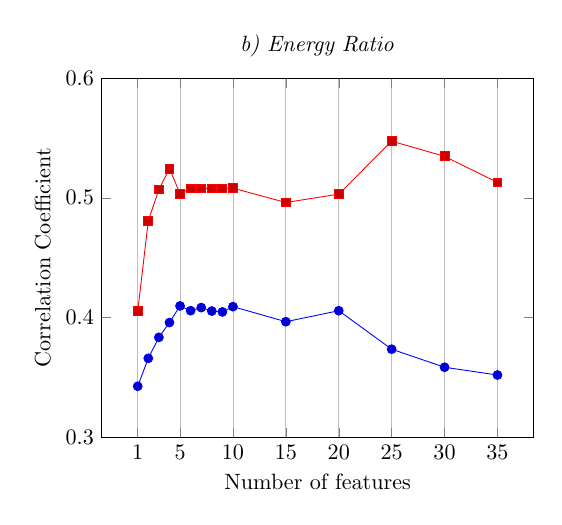
\begin{tikzpicture}[scale=0.8]

\begin{axis}[legend style={font=\scriptsize},
		title={\textit{b) Energy Ratio}},
        ylabel={Correlation Coefficient},
        xlabel={Number of features},
        ymin=0.30,ymax=0.60,
        xtick={1,5,10,15,20,25,30,35},
        xmajorgrids]

     \addplot coordinates { (1,0.3424) (2, 0.3658) (3, 0.3833) (4, 0.3957) (5, 0.4096) (6, 0.4056) (7, 0.4082) (8, 0.4053) (9, 0.4046) (10, 0.4090) (15, 0.3964) (20, 0.4056) (25, 0.3734) (30,0.3583) (35, 0.3518)};
     
     \addplot coordinates { (1, 0.4051) (2, 0.4808) (3, 0.507) (4, 0.5244) (5, 0.5035) (6, 0.5079) (7, 0.5079) (8, 0.5079) (9, 0.5079) (10, 0.5081) (15, 0.4961) (20, 0.5031) (25, 0.5474) (30, 0.5347) (35, 0.5129)};
    
  %  \addlegendentry{CrossValidation 10f}
   % \addlegendentry{Train dataset}

\end{axis}
\end{tikzpicture}

\caption[Results depending on the number of selected features.]{Results depending on the number of selected features according to table~\ref{tab:feature_selection}. Algorithm used: Decision Tree. Shown values correspond to Correlation Coefficients.}
\label{fig:feature_selection}
\end{figure}